\newpage
\section{Methodology}

Motivated by the previous examples, we propose OPTA, a new methodology for profiling energy consumption of tasks at runtime and dynamically adapting the energy budget to the varying energy consumption of tasks. 

\subsection{Online Profiling Method}

Here, we present an efficient online profiling method. 
OPTA dynamically profiles the actual voltage droop that a task consumes while the supply is connected. 
The actual voltage droop means the voltage droop in ${V_{cc}}$ by running a task if the supply current immediately drops to zero after the task starts. 
With the supply connected, the supply current keeps charging the capacitor during execution, so the actual voltage droop cannot be measured simply by two voltage measurements at the beginning and the end of a task. 
A naive solution will be disconnecting or short-circuiting the supply during profiling, but this can waste energy. 
In contrast, while keeping the supply connected, our method analyzes the supply current in the charge cycle, and uses it to derive the actual voltage droop in the discharge cycle. 
We will explain this method with its mathematical reasoning first, and then discuss possible concerns in its implementation. 

\subsubsection{Assumptions}

We have made the following assumptions for the mathematical reasoning. Later, we will discuss the situations where these assumptions do not hold.

\begin{itemize}
    \item \textit{The supply current remains constant across a charge-discharge cycle.} 
    In intermittently-powered systems, the energy buffering capacitor is typically small, e.g. tens to hundreds of \SI{}{\micro\farad}, and hence the charge-discharge cycle is typically short, e.g. tens to hundreds of \SI{}{\milli\second}. 
    The supply current is unlikely to change in such a short period. 
    Hence, in the following reasoning, we presume that the supply current is constant across a charge-discharge cycle. 

    \item \textit{The system is able to measure the supply voltage and time when active.} Off-the-shelf MCUs, e.g. MSP430 series, are equipped with many low-power peripherals, including ADC for measuring voltage and RTC for time-keeping. 
    In the following reasoning, we assume that these two modules are available and free of any overheads.
\end{itemize}

\subsubsection{Mathmatical Derivation}

\begin{figure}[!t]
    \centering
    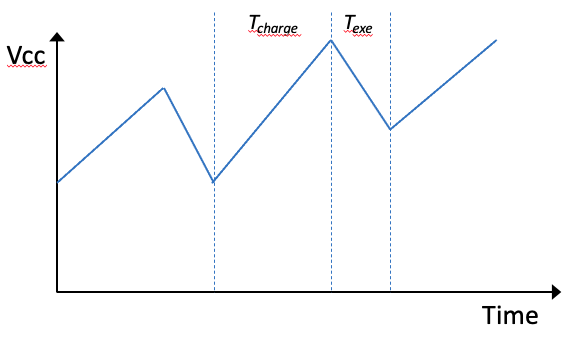
\includegraphics[width=3.49in]{ch5_repta/figures/math.jpg}
    \caption{Figure for illustrating mathematical derivation. }
    \label{fig:math}
\end{figure}

We show an illustrative trace of $V_{cc}$ across charge-discharge cycles in Fig.~\ref{fig:math}. 

(A list that explains math symbols to be inserted)

The charging cycle can be described as
\begin{equation}
    \Delta V_{charge} C = (I_{in} - I_{sleep}) T_{charge}
    \label{eq:vcharge} 
\end{equation}
where 
\begin{equation}
    I_{sleep} = I_{comp} + I_{rtc} + I_{lpm}
    \label{eq:isleep} 
\end{equation}

The discharging cycle can be described as
\begin{equation}
    \Delta V_{discharge} C = (I_{in} - I_{exe}) T_{discharge}
    \label{eq:vdischarge} 
\end{equation}
where
\begin{equation}
    I_{exe} = I_{comp} + I_{rtc} + I_{task}
    \label{eq:iexe} 
\end{equation}

The actual charge consumption of a task is
\begin{equation}
    \Delta V_{task} C = I_{exe} T_{discharge}
    \label{eq:vtaskc} 
\end{equation}

Combining (\ref{eq:vcharge}), (\ref{eq:isleep}), (\ref{eq:vdischarge}), (\ref{eq:iexe}), and (\ref{eq:vtaskc}), we can get the expression of $\Delta V_{task}$ as
\begin{equation}
    \Delta V_{task} = \Delta V_{charge} \frac{T_{exe}}{T_{charge}} - \Delta V_{exe} + \frac{I_{sleep}T_{exe}}{C}
    \label{eq:vtask} 
\end{equation}

Here, $\Delta V_{task}$ is the actual voltage droop that we should allocate before the execution of a task. 
$\Delta V_{charge}$, $\Delta V_{exe}$, $T_{exe}$, and $T_{charge}$ are the values that can be measured by the ADC and RTC at runtime. 
If $\frac{I_{sleep}T_{exe}}{C}$ is negligible, $\Delta V_{task}$ can be derived at runtime with all perceivable values. 

\subsubsection{Realistic Considerations}

Although the above equation is straightforward, there are some practical concerns that may affect the accuracy or efficiency. 

\begin{itemize}
    \item Minimizing $\frac{I_{sleep}T_{exe}}{C}$.

    As the profiling method ignores $\frac{I_{sleep}T_{exe}}{C}$, the profiled value can be theoretically smaller than the actual one. 
    However, if we look at the empirical values of $I_{sleep}$, $T_{exe}$, and $C$ in some typical IPSs, this is relatively small. 
    The sleep current $I_{sleep}$ is a key property that should be minimized in IPSs. 
    The execution time of a task $T_{exe}$ is typically within \SI{20}{\milli\second} as the energy storage capacitor cannot afford a long, energy-hungry task. 
    The capacitance of energy storage $C$ is usually from \SI{10}{\micro\farad} to hundreds of \SI{}{\micro\farad}. 
    Hence, $\frac{I_{sleep}T_{exe}}{C}$ is typically a few \SI{}{\milli\volt}. 
    This is insignificant compared to the voltage droop of a task (potentially hundreds of \SI{}{\milli\volt}), and is easily offset by a margin in implementation, e.g. the granularity of voltage comparator. 
    
    \item How fast can supply current change in a charge-discharge cycle? What can it cause?
    
    The rationale behind this method indicates that we use the average current input in the charge cycle as the current input in the discharge cycle. 
    Although this is unlikely to change largely considering the short execution time of a task, we still analyze the effect it can bring when the two current values are different. 
    We denote the two current values as $I_{in-charge}$ and $I_{in-discharge}$. 
    When $I_{in-charge} > I_{in-discharge}$, the system over-profiles the voltage droop. 
    This is typically fine, as the task can still safely finish and the over-profiled value would be corrected in the following measurements.
    When $I_{in-charge} < I_{in-discharge}$, the system under-profiles the voltage droop. 
    This can result in a lower energy budget than the safe one. 
    However, as $I_{in-discharge}$ is increasing, the task can usually finish with the additional energy. 
    The extreme case is when the system profiles a task with an increasing supply current, while executes the task with a decreasing supply current next time. 
    This can result in the failure of a task as it runs out of energy. 
    To maintain atomicity, our approach restarts the task from the beginning if it fails by disabling checkpoints during the task execution. 
    
    \item ADC, RTC, and processing overheads.
    
    The overheads of this profiling method in implementation come from ADC, RTC and processing.
\end{itemize}

\subsection{Threshold Adaptation}

\subsubsection{Profiling Strategy}

When should we take a profiling measurement?

Goal: Reduce unnecessary/redundant measurements and take necessary measurements.

\subsubsection{Learning Algorithm}

How do we use the measurements to update the voltage threshold?

Enable voltage threshold adaptation against runtime variation of energy consumption due to unforeseeable operating conditions, and also enable linear adaptation to function knobs that are known to the system. 

\begin{itemize}
    \item Without function knobs: use the latest profiled threshold.
    \item With function knobs: do a linear regression based on a number of recent measurements. 
\end{itemize}

